\documentclass{article}

% For figures
\usepackage{graphicx} 
\usepackage[figtopcap]{subfigure}

\usepackage{array} 

% For citations
\usepackage{natbib}

% For theorems
\usepackage{amsthm}

% For algorithms
\usepackage{algorithm,algorithmic}

\usepackage{hyperref}

% Packages hyperref and algorithmic misbehave sometimes.  We can fix
% this with the following command.
\newcommand{\theHalgorithm}{\arabic{algorithm}}

%\usepackage{icml2013} 
\usepackage[accepted]{icml2013}


% The \icmltitle you define below is probably too long as a header.
% Therefore, a short form for the running title is supplied here:
\icmltitlerunning{Spectral Experts}

% Math
\usepackage{amsmath,amssymb}
\usepackage{soul}

\providecommand{\Pa}{\textrm{Pa}}
\providecommand{\TensorFactorize}{\textsc{TensorFactorize}~}
\providecommand{\LearnFactors}{\textsc{LearnFactors}~}


% Section macros
\newcommand{\sectionref}[1] {\hyperref[#1]{Section \ref{#1}}}
\newcommand{\appendixref}[1] {\hyperref[#1]{Appendix \ref{#1}}}
\newcommand{\algorithmref}[1] {\hyperref[#1]{Algorithm \ref{#1}}}
\newcommand{\equationref}[1] {\hyperref[#1]{Equation \eqref{#1}}}
\newcommand{\figureref}[1] {\hyperref[#1]{Figure \ref{#1}}}
\newcommand{\tableref}[1] {\hyperref[#1]{Table \ref{#1}}}

\newtheorem{theorem}{Theorem}
\newtheorem{lemma}{Lemma}


% Matrix Perturbation
\newcommand{\inv}[1] {#1^{-1}}
\newcommand{\pinv}[1] {#1^{-\dagger}}
\newcommand{\Ap} {\hat{A}}
\newcommand{\Bp} {\hat{B}}
\newcommand{\Up} {\hat{U}}
\newcommand{\Vp} {\hat{V}}
\newcommand{\Xp} {\hat{X}}
\newcommand{\Wp} {\hat{W}}
\newcommand{\Zp} {\hat{Z}}
\newcommand{\vp} {\hat{v}}
\newcommand{\lambdap} {\hat{\lambda}}
\newcommand{\cnd}[1] {\kappa(#1)}
\newcommand{\aerr}[1] {\varepsilon_{#1}}
\newcommand{\rerr}[1] {\delta_{#1}}
\newcommand{\serr}[1] {\alpha_{#1}}
\newcommand{\gap}[1] {\Delta_{#1}}

% Keywords
\newcommand{\Pairs}{\mathrm{Pairs}}
\newcommand{\Triples}{\mathrm{Triples}}



%\DeclareMathSizes{8}{8}{6}{4}

\usepackage{etoolbox}
% This flag is used to include the appendix for the ArXiv version
\newtoggle{withappendix}
\toggletrue{withappendix}
%\togglefalse{withappendix}

\begin{document} 

\twocolumn[
%\icmltitle{Spectral Experts: A spectral algorithm for mixtures of linear regressions}
\icmltitle{Spectral Experts for Estimating Mixtures of Linear Regressions}
%\icmltitle{Efficient Consistent Estimation for Mixtures of Linear Regression}
%\icmltitle{Two Tensors Suffice: Efficient Consistent Estimation for Mixtures of Linear Regression}

% It is OKAY to include author information, even for blind
% submissions: the style file will automatically remove it for you
% unless you've provided the [accepted] option to the icml2013
% package.
\icmlauthor{Arun Tejasvi Chaganty}{chaganty@cs.stanford.edu}
\icmlauthor{Percy Liang}{pliang@cs.stanford.edu}
\icmladdress{Stanford University, Stanford, CA 94305 USA}

% You may provide any keywords that you 
% find helpful for describing your paper; these are used to populate 
% the "keywords" metadata in the PDF but will not be shown in the document
\icmlkeywords{spectral algorithms, mixture of experts, latent-variable
models, machine learning, ICML}

\vskip 0.3in
]

\begin{abstract}

Discriminative latent-variable models are typically learned using
EM or gradient-based optimization, which suffer from local optima.
In this paper, we develop a new computationally efficient
and provably consistent estimator for a mixture of linear regressions,
a simple instance of a discriminative latent-variable model.
Our approach relies on a low-rank linear regression to recover
a symmetric tensor, which can be factorized into the parameters
using a tensor power method.
We prove rates of convergence for our estimator
and provide an empirical evaluation illustrating
its strengths relative to local optimization (EM).

%  Spectral algorithms for latent variable models have seen considerable
%  recent interest for being efficient consistent estimators of model
%  parameters. These algorithms make few if any assumptions about the
%  generative process of the data, while providing a polynomial sample
%  and computational complexity. We present a new spectral algorithm for
%  a discriminative model, a mixture of linear regressions and show that
%  it can recover the regression coefficients with similar polynomial
%  guarantees. We evaluate the algorithm on linearly and non-linearly
%  generated data, as well as on a motion tracking task and compare it's
%  characteristics with an E-M algorithm.
\textbf{Last Modified: \today}
\end{abstract} 

\section{Introduction}
\label{sec:intro}

This is a sample article that uses the \textsf{jmlr} class with
the \texttt{wcp} class option.  Please follow the guidelines in
this sample document as it can help to reduce complications when
combining the articles into a book. Please avoid using obsolete
commands, such as \verb|\rm|, and obsolete packages, such as
\textsf{epsfig}.\footnote{See
\url{http://www.ctan.org/pkg/l2tabu}}

\section{Model}
\label{sec:model}

\newcommand{\xn}[1]{x^{(#1)}}
\newcommand{\xni}{\xn{i}}
\newcommand{\yn}[1]{y^{(#1)}}
\newcommand{\yni}{\yn{i}}

The mixture of linear regressions model describes response variables $y
\in \Re$ dependent on covariates $x \in \Re^d$ through $K$ different
modes which occur with probability $\pi_1, \dots, \pi_K$ respectively.
Each mode is independently described by regression coefficients
$\beta_k$ and we consider a common variance term $\sigma^2$. Given $x$,
the generative process for the response variables is,
\begin{eqnarray*}
  h &\sim& \mult(\pi) \\
  y | h = k &\sim& \normal{ \beta_{k}^T x}{ \sigma^2 },
\end{eqnarray*}
where $h$ is a latent variable corresponding to the mode.

Our learning framework can be described as follows; we observe $N$
samples, $(\xn{1}, \yn{1}), \dots, (\xn{N}, \yn{N})$ and would like to
recover the regressors, $B = [\beta_1 \mid \beta_2 \mid \cdots \mid
\beta_K]$, and the mixture probabilities, $\pi = (\pi_1, \pi_2, \dots,
\pi_K)$. Note that we do not observe $h$. If we did, the optimal
solution for $\beta_k$ would be the regressor found using least squares
on the set of points, $\{(x_i, y_i) | h_i = k \}$.


\section{Algorithm}
\label{sec:algo}

Recovery of $B$, $\mathcal{B}$.

Use AHK2012

Lemma error of $B$.

Lemma AHK2012 error

Theorem on polynomial recovery



%%%%%%%%%%%%%%%%%%%%%%%%%%%%%%%%%%%%%%%%%%%%%%%%%%%%%%%%%%%%
\section{Theoretical results}
\label{sec:theory}

In this section, we provide theoretical guarantees for the Spectral Experts algorithm.
Our main result shows that the parameter estimates $\hat\theta$ converge to $\theta$
at a $\frac{1}{\sqrt{n}}$ rate that depends polynomially on the bounds on the
parameters, covariates, and noise, as well the $k$-th smallest singular values
of the compound parameters and various covariance matrices.

\begin{theorem}[Convergence of Spectral Experts]
\label{thm:convergence}
Assume each dataset $\sD_p$ (for $p = 1, 2, 3$) consists of $n$ i.i.d.\ points independently drawn from a mixture
of linear regressions model with parameter $\theta^*$.\footnote{Having three independent copies simplifies the analysis.}
Further, assume 
$\|x\|_2 \le R$, 
$\|\beta_h^*\|_2 \le L$ for all $h \in [k]$,
$|\epsilon| \le S$
and $B$ is rank $k$.
Let $\Sigma_p \eqdef \E[\cvec(x\tp{p})\tp{2}]$, 
and assume $\Sigma_p \succ 0$ for each $p \in \{1,2,3\}$.
Let $\epsilon < \half$.
Suppose the number of samples is
$n = \max(n_1,n_2)$
where 
\begin{align*}
n_1 &= \Omega \left(\frac{R^{12} \log(1/\delta)}{\min_{p \in [3]} \sigmamin(\Sigma_p)^2} \right) \\
n_2 &= \Omega \left(\epsilon^{-2}~ \frac{k^2 \pi^2_{\max} \|M_2\|_\op^{1/2} \|M_3\|_\op^2 { L^{6} S^{6} R^{12}}}{\sigma_k(M_2)^{5} {\sigmamin(\Sigma_1)^2}} \log(1/\delta) \right).
\end{align*}
If each regularization strength $\lambda_n^{(p)}$ is set to 
$$\Theta\left( \frac{L^p S^p R^{2p}}{\sigmamin(\Sigma_1)^2} \sqrt{\frac{\log(1/\delta)}{n}} \right),$$
for $p \in 2, 3$,
%$O\left(\frac{\sigmamin(\Sigma_p)}{\sqrt{k}}~ \epsilon \right)$, 
%$\Omega\left(\sigma^3 L^3 R^6 \sqrt{\frac{\log(1/\delta)}{n}}\right)$,
then the parameter estimates $\hat\theta = (\hat\pi, \hat B)$ returned by
\algorithmref{algo:spectral-experts} (with the columns appropriately permuted)
satisfies 
  \begin{align*}
  \|\hat \pi - \pi \|_{\infty} \le \epsilon \quad\quad 
  %&= O\left(\frac{k \pi_{\max}^{5/2}\| {M_3} \|_\op}{\sigma_k(M_2)^{5/2}} ~ \epsilon \right) \\
  \|\hat \beta_h - \beta_h\|_2 \le \epsilon
  %&= O\left( \frac{k \pi_{\max} \|M_2\|_\op^{1/2} \| {M_3} \|_\op}{\sigma_k(M_2)^{5/2}}~ \epsilon \right),
  \end{align*}
  for all $h \in [k]$.
%$\|\hat\pi - \pi^*\|_{\infty} \le \epsilon$
%and for all $h \in [k]$,
%$\|\hat\beta_h - \beta^*_h\|_2 \le \frac{\epsilon}{\sqrt{\pi_h^*}}$.
\end{theorem}

While the dependence on some of the norms ($L^6,S^6,R^{12}$) looks formidable,
it is in some sense unavoidable, since we
need to perform regression on third-order moments.
Classically, the number of samples required is squared norm of the covariance matrix,
which itself is bounded by the squared norm of the data, $R^3$. This
third-order dependence also shows up in the regularization strengths;
the cubic terms bound each of $\epsilon^3$,
$\beta_h^3$ and $\|(x\tp{3})\tp{2}\|_F$ with high probability. 

The proof of the theorem has two parts.
First, we bound the error in the compound parameters estimates $\hat M_2,\hat M_3$
using results from \citet{Tomioka2011}.
Then we use results from \citet{AnandkumarGeHsu2012} to convert this error
into a bound on the actual parameter estimates $\hat\theta = (\hat\pi, \hat B)$
derived from the robust tensor power method.
But first, let us study a more basic property: identifiability.

%%%%%%%%%%%%%%%%%%%%%%%%%%%%%%%%%%%%%%%%%%%%%%%%%%%%%%%%%%%%

\subsection{Identifiability from moments}

In ordinary linear regression, the regression coefficients $\beta \in
\Re^d$ are identifiable if and only if the data has full rank:
$\E[x\tp{2}] \succ 0$, and furthermore, identifying $\beta$ requires
only moments $\E[xy]$ and $\E[x\tp{2}]$ (by observing the optimality
conditions for \refeqn{y1}).  However, in mixture of linear regressions,
these two moments only allow us to recover $M_1$.  \refthm{convergence}
shows that if we have the higher order analogues, $\E[x\tp{p}y\tp{p}]$
and $\E[x\tp{2p}]$ for $p \in \{1,2,3\}$, we can then identify the
parameters $\theta = (\pi, B)$,
provided the following \emph{identifiability condition} holds: $\E[\cvec(x\tp{p})\tp{2}] \succ
0$ for $p \in \{1,2,3\}$.

This identifiability condition warrants a little care,
as we can run into trouble when components of $x$ are dependent on each other
in a particular algebraic way.
For example, suppose $x = (1, t, t^2)$, the common polynomial
basis expansion, so that all the coordinates are deterministically
related.  While $\E[x\tp{2}] \succ 0$ might be satisfied (sufficient for ordinary linear regression),
$\E[\cvec(x\tp{2})\tp{2}]$ is singular for
any data distribution.
To see this, note that $\cvec(x\tp{2}) = [1 \cdot 1, t\cdot t, 2(1
\cdot t^2), 2(t \cdot t^2), (t^2 \cdot t^2)]$ contains components $t
\cdot t$ and $2(1 \cdot t^2)$, which are linearly dependent.  Therefore,
Spectral Experts would not be able to identify the parameters of
a mixture of linear regressions for this data distribution.

We can show that some amount of unidentifiability is intrinsic to
estimation from low-order moments, not just an artefact of our
estimation procedure.  Suppose $x = (t, \dots, t^d)$.  Even if we
observed all moments $\E[x\tp{p}y\tp{p}]$ and $\E[x\tp{2p}]$ for $p \in
[r]$ for some $r$, all the resulting coordinates would be monomials of $t$ up to only degree
$2dr$, and thus the moments live in a $2dr$-dimensional subspace.  On
the other hand, the parameters $\theta$ live in a subspace of at least
dimension $dk$.  Therefore, at least $r \ge k/2$ moments are required
for identifiability of any algorithm for this monomial example.

%%%%%%%%%%%%%%%%%%%%%%%%%%%%%%%%%%%%%%%%%%%%%%%%%%%%%%%%%%%%
\subsection{Analysis of low-rank regression}
\label{sec:regression}

In this section, we will bound the error of
the compound parameter estimates $\|\Delta_2\|_F^2$ and $\|\Delta_3\|_F^2$,
where $\Delta_2 \eqdef \hat M_2 - M_2$
and $\Delta_3 \eqdef \hat M_3 - M_3$.
Our analysis is based on the low-rank regression framework of
\citet{Tomioka2011} for tensors, which builds on
\citet{NegahbanWainwright2009} for matrices.
The main calculation involved is controlling the noise $\eta_p(x)$,
which involves various polynomial combinations of the mixing noise and observation noise.

Let us first establish some notation that unifies the three regressions (\refeqn{estimateM1}, \refeqn{estimateM2}, and \refeqn{estimateM3}).
Define the observation operator $\opX_p(M_p) : \Re^{d\tp{p}} \to \Re^{n}$
mapping compound parameters $M_p$:
\begin{align}
\opX_p(M_p; \sD)_i &\eqdef \innerp{M_p}{x\tp{p}_i}, & (x_i, y_i) \in \sD.
\end{align}

Let $\kappa(\opX_p)$ be the restricted strong convexity constant,
and let $\opX^*_p(\eta_p; \sD) = \sum_{(x,y) \in \sD} \eta_p(x) x\tp{p}$
be the adjoint.

%\paragraph{Restricted strong convexity}

%Let us first lower bound the restricted strong convexity constant
%$\kappa(\opX_p)$:

%In the previous section, we described an algorithm for the mixture of
%linear regressions using regression to recover $M_2$ and $M_3$,
%described by \equationref{eqn:y2} and \equationref{eq:y3}, as
%a subroutine. In this section, we will characterize the rate of
%convergence of regression.

%Analysis for regression in the fixed and random design settings have
%been studied before \citep{HsuKakadeZhang}, however our setup differs
%substantially from the noise models assumed in the literature. In our
%scenario, the variance in the estimation comes not only from the
%Gaussian observation noise (which has been studied before), but also
%from the variance in the latent variable $h$.

%Let us now formally define the class of regression problems we wish to
%analyze, i.e. regression on the set $(x\tp{p}, y^p)$,
%\begin{align*}
%  y^p &= \innerp{x\tp{p}}{M_p} + (\innerp{x\tp{p}}{M_p - \beta_h\tp{p}} + \varepsilon).
%\end{align*}

%\todo{Describe/define the convex tensor stuff.}
%We would like to exploit
%the property that $M_p$ is low rank (as typically $k \ll D$). It has
%been shown that a convex relaxation for this problem regression with
%trace norm regularization, which can be solved using a proximal
%subgradient descent algorithm\citationneeded.
%The analogue of trace norm
%regularization for higher order tensors corresponds to the sum of the
%trace norms of the mode-k unfolding of the tensor \cite{Tomioka2011},
%$X_{(k)}$, is a $d_k \times (\prod_{k' \neq k} d_{k'})$ matrix obtained
%by concatenating the entries for all dimensions other than $k$. For
%example, the 1-mode unfolding of a 3rd order tensor has entries,
%$X_{(1)}^{i_1, (i_2, i_3)} = X_{i_1, i_2, i_3}$.

%In general, the optimization problem we'd like to solve is,
%\begin{align}
%  \hat M_p &= 
%  \arg\min_{M_p}& \frac{1}{2N} \| \vec y - \opX_p(M_p) \|_2^2 + \frac{\lambda_n}{k} \sum_{h=1}^k \| (M_p)_{(h)} \|_* \label{eq:regression}.
%\end{align}

\begin{lemma}[\citet{Tomioka2011}, Theorem 1]
\label{lem:lowRank}
Suppose there exists a restricted strong convexity constant $\kappa(\opX_p)$ such that
$$\frac{1}{n} \| \opX_p( \Delta )\|_2^2 \ge \kappa(\opX_p) \|\Delta\|^2_F \quad \text{and} \quad
\lambda^{(p)}_n \ge \frac{2 \|\opX_p^*(\eta_p)\|_\op}{n}.$$
Then the error of $\hat M_p$ is bounded as follows:
$$\| \hat M_p - M_p \|_F \le \frac{32 \lambda^{(p)}_n \sqrt{k}}{\kappa(\opX_p)}.$$
\end{lemma}

Going forward, we need to lower bound the restricted strong convexity
constant $\kappa(\opX_p)$ and upper bound the operator norm of the adjoint operator
$\|\opX_p^*(\eta_p)\|_\op$. The proofs of the following lemmas follow
from standard concentration inequalities and are detailed in 
\iftoggle{withappendix}{
\appendixref{sec:proofs:regression}.
}{
the supplementary material.
}
%have been deferred to \appendixref{sec:proofs}. 

%We will appeal to the random design framework that models the input $x$
%as random and show bounds that hold with high probability.
%\paragraph{Adjoint operator}
%In this section, we upper bound the operator norm of the adjoint
%$\|\opX_p(\eta_p)\|_\op$.

% First, let us lower bound the restricted strong convexity parameter $\kappa(\opX_p)$:

\begin{lemma}[lower bound on restricted strong convexity constant]
\label{lem:lowRankLower}
%Let $\Sigma_p \eqdef \E[\cvec(x\tp{p})\tp{2}]$.
If $$n = \Omega \left(\max_{p\in [3]} \frac{R^{4p} (p!)^2 \log(1/\delta)}{\sigmamin(\Sigma_p)^2} \right),$$
then with probability at least $1-\delta$:
$$\kappa(\opX_p) \ge \frac{\sigmamin(\Sigma_p)}{2},$$
for each $p \in [3]$.
\end{lemma}

% Next, let us upper bound the operator norm of the observation adjoint:

\begin{lemma}[upper bound on adjoint operator]
\label{lem:lowRankUpper}
% Let $\opX_p$ be the linear operator previously defined. 
If $$n = \Omega \left(\max_{p\in [3]} \frac{L^{2p} S^{2p} R^{4p} \log(1/\delta)}{ \sigmamin(\Sigma_1)^2 \left(\lambda_n^{(p)}\right)^2} \right),$$
then with probability at least $1-\delta$:
$$\lambda_n^{(p)} \ge \frac1{n} \|\opX_p^*(\eta_p)\|_\op,$$
for each $p \in [3]$.
\end{lemma}

%%%%%%%%%%%%%%%%%%%%%%%%%%%%%%%%%%%%%%%%%%%%%%%%%%%%%%%%%%%%
\subsection{Analysis of the tensor factorization} 
\label{sec:tensorError}

Having bounded the error of the compound parameter estimates $\hat M_2$ and $\hat M_3$,
we will now study how this error propagates through the tensor factorization step of 
\algorithmref{algo:spectral-experts},
which includes whitening, applying the robust tensor power method \cite{AnandkumarGeHsu2012},
and unwhitening.
\begin{lemma}
  \label{lem:tensorPower}
  Let $M_3 = \sum_{h=1}^{k} \pi_h \beta_h\tp{3}$.
  Let $\|\hat M_2 - M_2\|_\op$ and $\|\hat M_3 - M_3\|_\op$ both be less than
  \vspace{-0.5em}
  $$\frac{\sigma_k(M_2)^{5/2}}{k \pi_{\max} \|M_2\|_\op^{1/2} \| {M_3} \|_\op}~ \epsilon,$$
  for some $\epsilon < \half$. 
  Then, there exists a permutation of indices such that  the parameter
  estimates found in step 2 of \algorithmref{algo:spectral-experts}
  satisfy the following with probability at least $1 - \delta$:
  \begin{align*}
  \|\hat \pi - \pi \|_{\infty} &\le \epsilon \\
  %&= O\left(\frac{k \pi_{\max}^{5/2}\| {M_3} \|_\op}{\sigma_k(M_2)^{5/2}} ~ \epsilon \right) \\
  \|\hat \beta_h - \beta_h\|_2 &\le \epsilon.
  %&= O\left( \frac{k \pi_{\max} \|M_2\|_\op^{1/2} \| {M_3} \|_\op}{ \sigma_k(M_2)^{5/2} }~ \epsilon \right),
  \end{align*}
  for all $h \in [k]$.
\end{lemma}

The proof follows by applying standard matrix perturbation results for
the whitening and unwhitening operators and 
\iftoggle{withappendix}{
can be found in \appendixref{sec:proofs:tensors}.
}{
has again been deferred to the supplementary material.
}
%\appendixref{sec:proofs}. 

%%%%%%%%%%%%%%%%%%%%%%%%%%%%%%%%%%%%%%%%%%%%%%%%%%%%%%%%%%%%
\subsection{Synthesis}
Together, these lemmas allow us to control the compound parameter error
and the recovery error. We now apply them in the proof of
\refthm{convergence}:

\begin{proof}[Proof of Theorem 1 (sketch)]
By \reflem{lowRank}, \reflem{lowRankLower} and \reflem{lowRankUpper}, we
can control the Frobenius norm of the error in the moments, which
directly upper bounds the operator norm: If $n \ge \max\{n_1, n_2\}$,
then
\begin{align}
  \|\hat M_p - M_p\|_\op = O\left( \lambda_n^{(p)} \sqrt{k} \sigmamin(\Sigma_p)^{-1} \right).
  %\|\hat M_p - M_p\|_\op = O\left( \sigma^3 L^3 R^6 k^{\frac12} \sigmamin(\Sigma_p)^{-1} \sqrt{\frac{\log^3 (1/\delta)}{n}} \right).
  %\|\hat M_p - M_p\|_F = O\left( \frac{\sigma^3 L^3 R^6 \sqrt{k} \log^3 (1/\delta)}{\sqrt{n} (\sigmamin(\Sigma_p) - d^p R^p \sqrt{\frac{p \log(d) \log(1/\delta)}{n}}} \right).
\end{align}

We complete the proof by applying \reflem{tensorPower} with the above
bound on $\|\hat M_p - M_p\|_\op$.

\end{proof}


%\subsection{Low-rank Regression}
\label{sec:regression}

The goal of this section is to bound the error of
the compound parameter estimates,
specifically $\|\Delta_2\|_F^2$ and $\|\Delta_3\|_F^2$,
where $\Delta_2 \eqdef \hat M_2 - M_2$
and $\Delta_3 \eqdef \hat M_3 - M_3$.

Our analysis is based on the low-rank regression framework of
\citet{Tomioka2011} for tensors, which builds off of
\citet{NegahbanWainwright2009} for matrices.
Define the observation operator $\opX(M_p) : \Re^{d\tp{p}} \to \Re^{n}$
mapping compound parameters $M_p$:
\begin{align}
  \opX(M_p; \sD)_i &\eqdef \frac12 \sum_{(x,y) \in \sD} \innerp{M_p}{x\tp{p}}_i, \quad i  \in [n].
\end{align}

Let $\kappa(\opX)$ be the restricted strong constant,
and let $\opX^*(\eta_p; \sD) = \sum_{(x,y) \in \sD} \eta_p(x) x\tp{p}$
be the adjoint.

\paragraph{Restricted strong convexity}

In this section, we compute the restricted strong convexity constant
$\kappa(\opX)$ for our problem.

%In the previous section, we described an algorithm for the mixture of
%linear regressions using regression to recover $M_2$ and $M_3$,
%described by \equationref{eqn:y2} and \equationref{eq:y3}, as
%a subroutine. In this section, we will characterize the rate of
%convergence of regression.

%Analysis for regression in the fixed and random design settings have
%been studied before \citep{HsuKakadeZhang}, however our setup differs
%substantially from the noise models assumed in the literature. In our
%scenario, the variance in the estimation comes not only from the
%Gaussian observation noise (which has been studied before), but also
%from the variance in the latent variable $h$.

%Let us now formally define the class of regression problems we wish to
%analyze, i.e. regression on the set $(x\tp{p}, y^p)$,
%\begin{align*}
%  y^p &= \innerp{x\tp{p}}{M_p} + (\innerp{x\tp{p}}{M_p - \beta_h\tp{p}} + \varepsilon).
%\end{align*}

%\todo{Describe/define the convex tensor stuff.}
%We would like to exploit
%the property that $M_p$ is low rank (as typically $K \ll D$). It has
%been shown that a convex relaxation for this problem regression with
%trace norm regularization, which can be solved using a proximal
%subgradient descent algorithm\citationneeded.
%The analogue of trace norm
%regularization for higher order tensors corresponds to the sum of the
%trace norms of the mode-k unfolding of the tensor \cite{Tomioka2011},
%$X_{(k)}$, is a $d_k \times (\prod_{k' \neq k} d_{k'})$ matrix obtained
%by concatenating the entries for all dimensions other than $k$. For
%example, the 1-mode unfolding of a 3rd order tensor has entries,
%$X_{(1)}^{i_1, (i_2, i_3)} = X_{i_1, i_2, i_3}$.

%In general, the optimization problem we'd like to solve is,
%\begin{align}
%  \hat M_p &= 
%  \arg\min_{M_p}& \frac{1}{2N} \| \vec y - \opX(M_p) \|_2^2 + \frac{\lambda_n}{K} \sum_{h=1}^K \| (M_p)_{(h)} \|_* \label{eq:regression}.
%\end{align}

%We begin our analysis by stating a generic theorem about convex
%optimization problem in \equationref{eq:regression}, 
\begin{lemma}[convergence of low-rank regression]
If restricted strong convexity holds
$$\frac{1}{2n} \| \opX( \Delta )\|_2^2 \ge \kappa(\opX) \|\Delta\|^2_F \quad \text{and} \quad
\lambda_n \ge \frac{|\opX^*(\eta_p)|}{n}.$$
Then the error of $\hat M_p$ is bounded as follows:
$\| \hat M_p - M_p^* \|_F \le \frac{\lambda_n \sqrt{k}}{\kappa(\opX)}$.
\end{lemma}
\begin{proof}
  \citet{Tomioka2011}, Theorem 1.

  This proof follows from convex properties \todo{elaborate}.
  \citet{NegahbanWainwright2009} prove this theorem for matrices, i.e.
  when $p = 2$. \citet{Tomioka2011} generalized it for arbitrary $p$.
\end{proof}

Going forward, we need to lower bound the restricted strong convexity
parameter $\kappa(\opX)$ and upper bound the adjoint operator
$\|\opX^*(\epsilon)\|_{2}^2$, which corresponds to a gradient update. We
will appeal to the random design framework that models the input $x$ as
random and show bounds that hold with high probability.

\begin{lemma}[restricted strong convexity]
Let $\opX$ be the linear operator previously defined. Then,
$$\kappa(\opX) \ge Y$$.
\end{lemma}
\begin{proof}
  \todo{Do I need to transform rewrite $M_p$ in terms of orthogonal components?}

  \begin{align*}
    \frac{\|\opX(M_p)\|_1}{N} &= \frac{1}{N}\sum_{i=1}^{N} |\innerp{x_i\tp{p}}{M_p}| \\
    &\ge \frac{1}{N}\sum_{i=1}^{N} \sigma_{min}( M_p ) \|x_i\|^p \\
    &\ge \frac{\kappa(M_p)}{\sqrt{D}} \frac{\sum_{i=1}^{N} \|x_i\|^p}{N} \| M_p \|_F.
  \end{align*}

  While $\kappa(M_p)$ depends on $M_p$ we can lower bound it by
  restricting the convex space to $\{ M_p | \kappa(M_p) \ge \kappa \}$.
  Further, using concentration bounds, we can lower bound $\|x_i\|^p$ as
  well. \todo{What is $\E[\|x_i\|^3]$? It is some quantity greater than
  zero}.
  
  Thus, 
  \begin{align*}
  \frac{ \|\opX(M_p)\|_2 }{2 N} 
  &\ge
  \frac{ \|\opX(M_p)\|_1 }{2 \sqrt{D}N} 
  &\ge \frac{\kappa}{2 D} (\E[\|x_i\|^p] - \frac{t}{N}) \| M_p \|_F.
  \end{align*}
  with high probability $1 - \delta$. \todo{The bound needs to be shown
  for $\| \opX(M_p) \|_2^2$.}
  
  In other words, $\kappa(\opX)
  = \frac{\kappa}{2 D} (\E[\|x_i\|^p] - \frac{t}{N})$ is a valid
  lower bound.
\end{proof}

By Lemma 19 of \cite{hsu13spherical},
we have that $\frac{1}{n} \sum_{i=1}^n \epsilon_i^3 = O(\sqrt{\frac{\log^3(1/\delta)}{n}})$.
with probability at least $1-\delta$.

\begin{lemma}[bounded error]
  Let $\opX$ be the linear operator previously defined. Then,
  $$\opX^*(\epsilon) \le Y$$.
\end{lemma}
\begin{proof}
  \begin{align*}
    \frac{\opX^*(\epsilon)}{N} 
    &= \frac{1}{N}\sum_{i=1}^{N} \epsilon_i \innerp{x_i\tp{p}}{M_p} \\
    &= \frac{1}{N}\sum_{i=1}^{N} (\innerp{x_i\tp{p}}{M_p - \beta_i\tp{p}} + \varepsilon)  \innerp{x_i\tp{p}}{M_p}.
  \end{align*}
  Let $M_p - \beta_i\tp{p} = \tilde M_i$ and consider it to be a random
  variable.
  \begin{align*}
    \frac{\opX^*(\epsilon)}{N} 
    &= \frac{1}{N}\sum_{i=1}^{N} \innerp{\tilde M_i}{x_i\tp{2p}} + \varepsilon \innerp{M_p}{x_i\tp{p}} \\
    &\le \frac{1}{N}\sum_{i=1}^{N} \|\tilde M_i\|_{op} \|x_i\|^{2p} + \varepsilon \|M_p\|_{op}\|x_i\|^{p} \\
    &\le \|M_p\|_{op} ( \frac{1}{N}\sum_{i=1}^{N} \|x_i\|^{2p} + \varepsilon \|x_i\|^{p} ).
  \end{align*}

  We can probabilistically bound the above by considering the union
  bound of $\varepsilon$ and $\|x_i\|^p$.


  Finally,
  \begin{align*}
    \frac{\opX^*(\epsilon)}{N} 
    &\le \|M_p\|_{op} (\E[\|x_i\|^{2p}] + t/N + (t/N) (\E[ \|x_i\|^{p} ] + t/N) ),
  \end{align*}
  with high probability. Note that this does not converge to $0$ as $N
  \to \infty$ because of the variance of the selection probability.
\end{proof}
 % Integrated into theory
%\subsection{Tensor Factorization}
\label{sec:tensor-power}

Write out the form of $B$ and $\mathcal{B}$ in symmetric tensor form.

Use Tensor Power Method to recovery $\beta_k$.

\begin{lemma}
  Let $\hat T = T + E$, where $T$ is a symmetric tensor with orthogonal decomposition $T = \sum_{i=1}^k \lambda_i v_i\tp{3}$ and each $\lambda_i > 0$. If 
  \begin{align}
    \epsilon &\le O(\frac{\lambda_{min}}{k}) \\
    N &\ge O(\log(k) + \log \log(\frac{ \lambda_{max} }{\epsilon} ), 
  \end{align}
  and for $L = O( poly(k) \log(\frac{1/\eta}) )$  attempts, then with
  probability atleast $1 - \eta$, there exists a permutation $\pi$ on
  $[k]$ such that,
  \begin{align}
    \|v_{\pi(j)} - \hat v_j\| &\le 8 \epsilon/\lambda_{\pi(j)} \\
    \|\lambda_{\pi(j)} - \hat \lambda_j\| &\le 5 \epsilon.
  \end{align}
\end{lemma}
\begin{proof}
  \cite{AnandkumarGeHsu2012}
\end{proof}

\todo{ This only gives us the eigenvectors for an orthogonal
decomposition. We also need to work out the darned coefficients
whitening the tensor adds.  Namely, what is $\delta T(W,W,W)$ (for which
the above bound applies), given $\delta W$ and ultimately $\delta P$
($W^T P W = I$). These calculations can be found in the notes I had had
earlier.}

 % Integrated into theory
\section{Empirical Evaluation}
\label{sec:evaluation}

\todo{Fill it up with juicy bits once we actually have them graphs.}

\subsection{Experimental Setup}

\paragraph{Algorithms}

We implemented the low rank recovery optimization routines for $M_2$ and
$M_3$ using a proximal subgradient descent algorithm\citationneeded. The
algorithm was initialized with the regularized least squares solution
and was run to convergence in each instance. Both regularization
parameters, $\lambda_n^{(2)}$ and, $\lambda_n^{(3)}$ were annealed as
$\frac{1}{n}$. 

As a baseline, we also implemented EM with two different
initializations. In the first, we used $\beta$s with random standard
Gaussian entries and uniform mixture probabilities, $\pi$. In the other,
we initialized EM with the starting points given by Spectral Experts. 

\paragraph{Datasets}

We generated synthetic data using covariates from the unit hyper cube
and non-linear responses.  To conform to the identifiability criteria
discussed in \sectionref{sec:algo}, we considered only features that
would guarantee this condition. 

As an example, one set of features we considered in the uni-dimensional
setting were $\{1, x, x^4, x^7\}$. The data and the curves fit using
Spectral Experts, EM with random initializations and EM initialized with
the parameters recovered using spectral experts are shown in
\figureref{fig:curves}.

\begin{figure*}[t]
  \centering
  \subfigure[Spectral]{
    \includegraphics[width=0.50\textwidth]{figures/curves-vis/1-8-3-specm.pdf}}
    \hspace{-2em}
  \subfigure[EM]{
    \includegraphics[width=0.50\textwidth]{figures/curves-vis/1-8-3-em.pdf}}
%  \subfigure[Spectral + EM]{
%    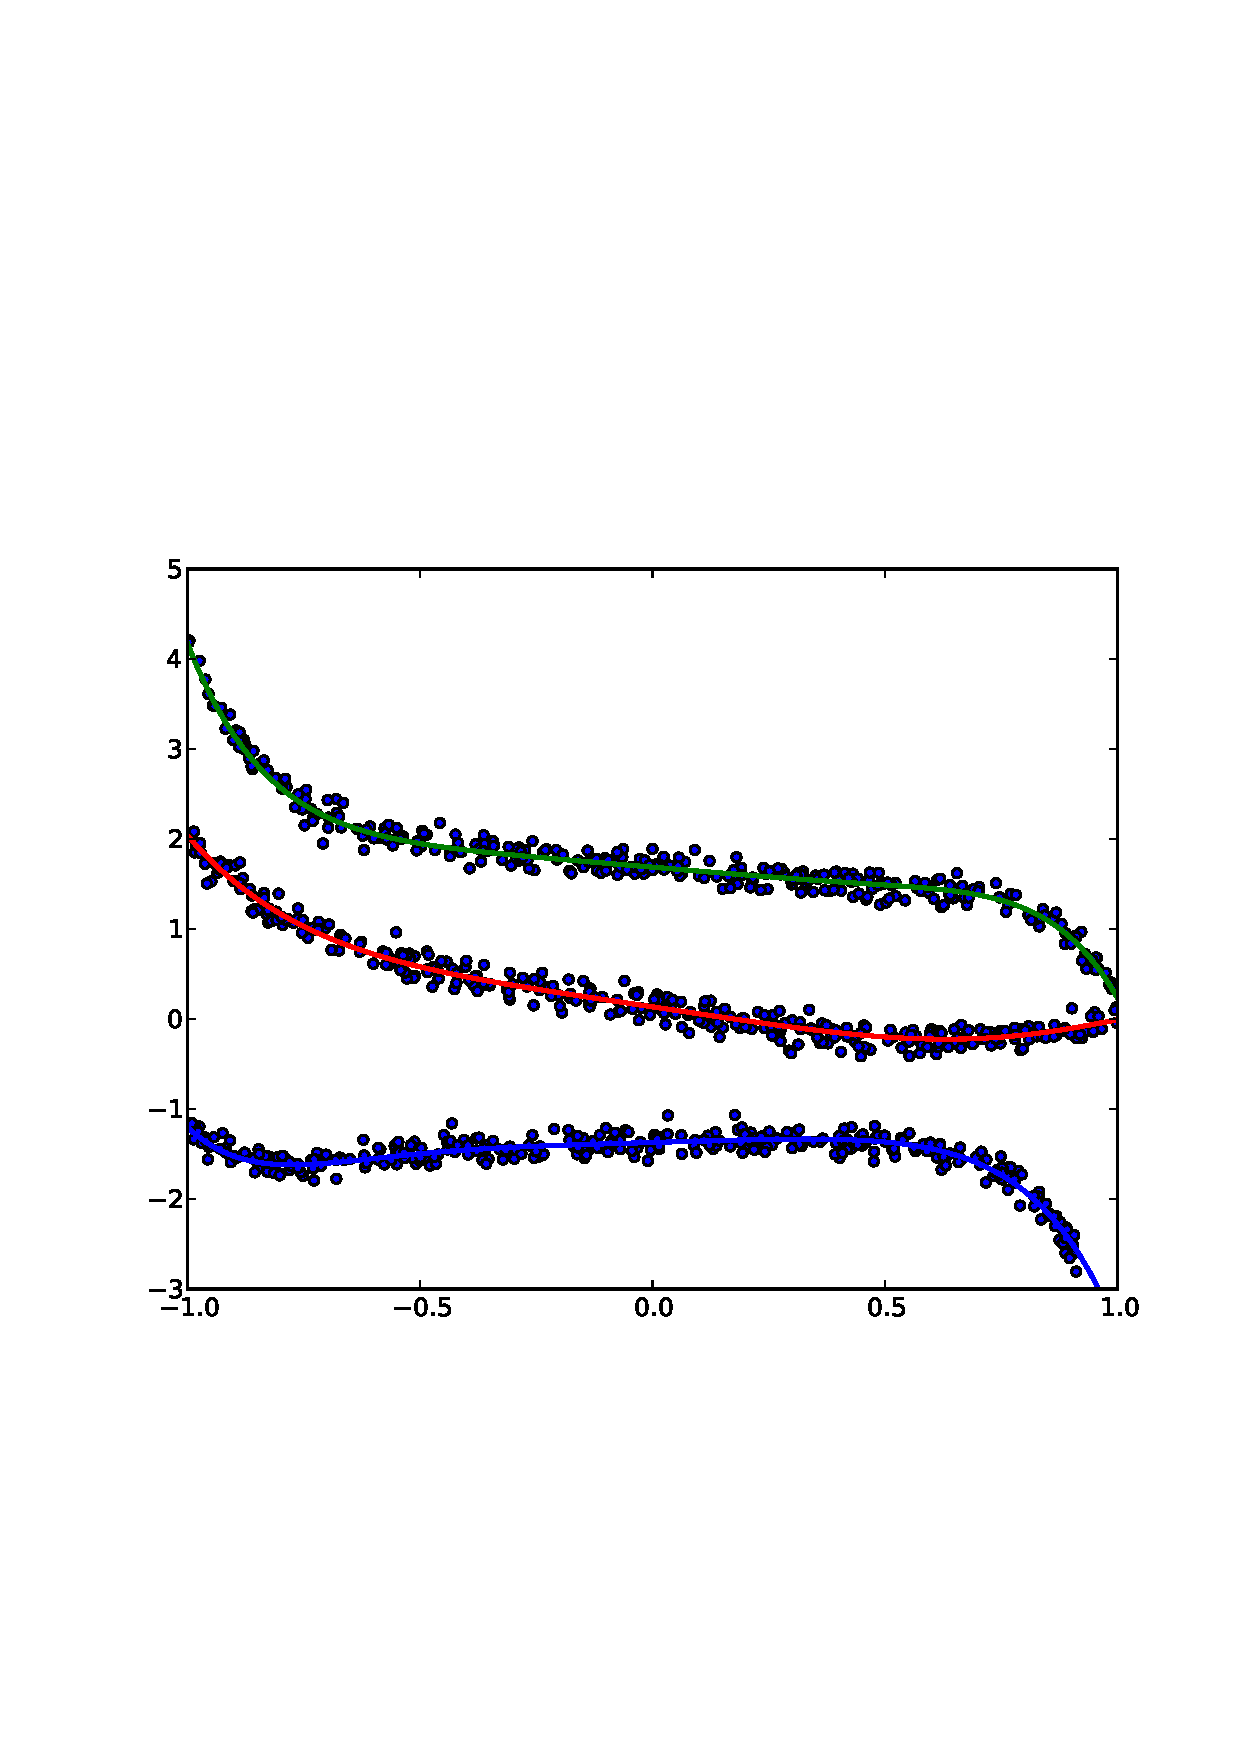
\includegraphics[width=0.34\textwidth]{figures/curves-vis/1-8-3-spem.png}}
  \caption{A comparison between SpectralExperts and EM. The dashed lines
  on the left denote the solution recovered by Spectral Experts. Whilst
  not a perfect fit, it provides an good initialization for EM to find
  the true global minima. The dotted lines on the right show different
  local optima found by EM on this example.}
  \label{fig:curves}
\end{figure*}

%Default values:
%$n = 10^6$
%$k = 5$

\begin{table*}[t]
\caption{Parameter Recovery ($N = 500,000$).}
\label{tbl:parameter-recovery}
\vskip 0.15in
\begin{center}
\begin{small}
\begin{sc}

  \begin{tabular}{ >{\centering}p{5cm}<{\centering} r c c c }
\hline
\abovespace\belowspace
Features  & $K$ & Spectral & EM & Spectral + EM \\
\hline
\abovespace
$\{1$, $ x_1$, $ x_1^4\}$ 
  & 2 & 1.52 $\pm$ 0.71 & 0.28 $\pm$ 0.82 & {\bf 0.13 $\pm$ 0.55} \\
$\{1$, $ x_1$, $ x_2$, $ x_1^2 x_2^2\}$ 
  & 3 & 1.87 $\pm$ 1.20 & {\bf 0.33 $\pm$ 0.96} & 0.35 $\pm$ 1.23 \\
$\{1$, $ x_1$, $ x_2$, $ x_1 x_2^3$, $ x_1^2 x_2^2$, $ x_1^3 x_2 \}$ 
& 5 & 5.27 $\pm$ 2.32 & 1.80 $\pm$ 1.80 & {\bf 1.51 $\pm$ 1.77} \\
$\{1$, $ x_1$, $ x_2$, $ x_1 x_2^3$, $ x_1^2 x_2^2$, $ x_1^3 x_2$, $ x_1^3 x_2^4$, $ x_1^4 x_2^3 \}$ 
& 7 & 8.42 $\pm$ 1.66 & 7.41 $\pm$ 2.99 & {\bf 7.31 $\pm$ 2.47} \\
$\{1$, $ x_1$, $ x_2$, $ x_3$, $ x_1 x_2 x_3^2$, $ x_1 x_2^2 x_3$, $ x_1^2 x_2 x_3$, $ x_1^2 x_2^2$, $ x_1^2 x_3^2$, $ x_2^2 x_3^2$, $ x_3^2\}$
& 3 & 3.78 $\pm$ 0.90 & 0.67 $\pm$ 1.49 & {\bf 0.51 $\pm$ 1.12} \\
$\{1$, $ x_1$, $ x_2$, $ x_3$, $ x_1 x_2 x_3^2$, $ x_1 x_2^2 x_3$, $ x_1^2 x_2 x_3$, $ x_1^2 x_2^2$, $ x_1^2 x_3^2$, $ x_2^2 x_3^2$, $ x_3^2\}$
  & 7 & 9.97 $\pm$ 3.22 & 1.43 $\pm$ 1.97 & {\bf 1.42 $\pm$ 2.17} \\
\hline
\end{tabular}
\end{sc}
\end{small}
\end{center}
\vskip -0.1in
\end{table*}

% \todo{Dataset 2: $b = 30$, $p = 1$. I'm unclear as to what we can show
% on this sort of data set. EM works extremely well, and the spectral
% methods do not converge easily.}

\subsection{Results}

\tableref{tbl:parameter-recovery} presents the Fro\"ebenius norm of the
difference between true and estimated parameters for the model, averaged
over 20 different random instances for each feature set and 10 attempts
for each instance. The experiments were run using $N = 500,000$ samples.

There is a lot of variation across random instances; some are easy for
EM to find the global minima and others more difficult. Moreover, simply
increasing the number of samples did not necessarily improve EM
performance. In general, we found that while our spectral algorithm did
not recover parameters extremely well, it provided a good initialization
for EM. 

\todo{Plot: the histogram over errors (for EM?) Some plots I have
doesn't really show much}.

\paragraph{Misspecified Data}

To evaluate how robust the algorithm was to model mis-specification, we
removed large contiguous sections from $x \in [-0.5,-0.25] \cup
[0.25,0.5]$. The lower half of \tableref{tbl:parameter-recovery} reports
recovery errors in this scenario. 

\paragraph{Effect of number of data points}

\begin{figure*}[t]
  \centering
  \subfigure[Complete Data]{
    \includegraphics[width=0.50\textwidth]{figures/vs-n/1-8-3-3.pdf}
  }
    \hspace{-2em}
  \subfigure[Incomplete Data]{
    \includegraphics[width=0.50\textwidth]{figures/vs-n/1-8-3-3-rm.pdf}
  }
  \caption{}
  \label{fig:vs-n}
\end{figure*}

Highlight



\todo{We see that the error of spectral is actually less than EM after a point.}

Point: tradeoff between statistical error and computational error;
not enough data, spectral is actually a lot worse
given enough data, spectral+EM is much better

\paragraph{Effect of noise}

\paragraph{Effect of separation between components}

\section{Discussion}
\label{sec:discussion}

% Summarize paper
For latent-variable models,
there has been tension between
local optimization of likelihood,
which is broadly applicable but offers no global theoretical guarantees,
and the spectral method of moments, which provides consistent estimators
but are limited to models with special structure.
The purpose of this work is to show that the two methods
can be used synergistically to produce consistent estimates
for a broader class of directed and undirected models.
%for example, undirected log-linear models with high treewidth.

% Bottleneck is key: previous work is preprocessing
Our approach provides consistent estimates for
a family of models in which each hidden variable is a \emph{bottleneck}---that is,
it has three conditionally independent observations.
This bottleneck property of \citet{anandkumar13tensor}
has been exploited in many other contexts,
including Latent Dirichlet Allocation \cite{anandkumar12lda},
mixture of spherical Gaussians \cite{hsu13spherical},
probabilistic grammars \cite{hsu12identifiability},
noisy-or Bayesian networks \cite{halpern2013unsupervised},
mixture of linear regressions \cite{chaganty13regression},
and others.
Each of these methods can be viewed as ``preprocessing'' the given model into a
form that exposes the bottleneck or tensor factorization structure.
The model parameters correspond directly to the solution of the factorization.

% Our work: post-processing
In contrast, the bottlenecks in our graphical models are given by assumption,
but the conditional distribution of the observations given the bottleneck
can be quite complex.
Our work can therefore be viewed as ``postprocessing'',
where the conditional moments recovered from tensor factorization
are used to further obtain the hidden marginals and eventually the parameters.
Along the way, we developed the notion of exclusive views and bidependent sets,
which characterize conditions under which the conditional moments can reveal
the dependency structure between hidden variables.
We also made use of custom likelihood functions which were constructed to be
easy to optimize.

%We also show that bottlenecks lead to a notion of \emph{exclusive views}
%(\definitionref{exclusive-views}), the key property that allows us to learn the
%correlation structure between hidden variables.

%Much recent work on method of moments for estimating latent-variable models
%has focused on increasing applicability to broader range of models,

%In this paper, we we've described an algorithm that can consistently
%  estimate parameters for the class of directed and undirected graphical
%  models for which each hidden variable has at least three conditionally
%  independent observed variables (\propertyref{bottleneck}).

%This condition is sufficiently general to capture a variety of popular
  %models like latent trees and grids (like a pairwise latent Markov random field).
%The undirected model setting applies to log-linear models, allowing
%  for discriminative featurization; furthermore, in practice, the
%  bottleneck condition can be enforced on a model if the observed
%  features can be split into two uncorrelated sets.

% Correlation structure
%Other authors \citep{anandkumar12lda, anandkumar2013linear,
%  halpern13noisyor} learn parameters for models outside our
%  family, but they do so with additional knowledge of the correlation structure
%  between hidden variables, allowing them to ``subtract'' out these correlations and
%  obtain a graph that is bottlenecked.
% TOO BOLD
%Thus, while \propertyref{bottleneck} is much stronger than
%  \propertyref{exclusive-views}, we expect that without any knowledge of
%  the correlation between variables, \propertyref{bottleneck} is
%  necessary for identifiability.
%Our work uses the \TensorFactorize algorithm presented by
%  \citet{anandkumar13tensor}, first
%  studied the consistent parameter estimation algorithm for the
%  three-view mixture model.
%
%\todo{What about Mossel and Roch?}
%For example,
%\citet{anandkumar12lda} are able to recover parameters for correlated
%  discrete mixtures, e.g. latent Dirichlet allocation; their approach
%  follows that of the three-view mixture model, with a pre-processing step
%  that subtracts the correlation between the views.
%\citet{anandkumar2013linear} study a special family of Bayesian networks
%  in which the observed variables are linearly related to a sparse set of
%  hidden variables. Once again, the key step is to identify the
%  correlations between observed variables and exclude them from the views.
%\citet{halpern13noisyor} propose an algorithm to recover factors for
%  a more densely connected bipartite noisy-or network; they also use
%  bottlenecks to learn parameters, but exploit properties of the model
%  to negate correlations from learned edges, allowing for more
%  bottlenecks to be discovered. 
%Our work makes a different tradeoff: we do not assume any special correlation structure,
%but do rely on every hidden variable having an exclusive view so that we can
%learn the underlying structure.

%work to settings that do not meet the
  %criterion \propertyref{bottleneck}, but rely on knowing more about
  %the underlying correlation structure of the problem.
%In comparison, our work applies to a general family of models, including
%  latent tree models, directed and undirected grids, with no assumptions
%  on the correlation structure aside from independences encoded in the
%  graph. 

% Observable operator
Another prominent line of work in the method of moments community has
  focused on recovering {\em observable operator
  representations} \citep{jaeger2000observable,hsu09spectral,bailly2010spectral,balle12automata}.
  These methods allow prediction of new observations, but do not
  recover the actual parameters of the model, making them difficult to use
  in conjunction with likelihood-based models. % which are driven by parameters.
\citet{song2011spectral} proposed an algorithm to learn observable
  operator representations for latent tree graphical models, like the
  one in \figureref{examples-tree}, assuming the graph is bottlenecked. 
Their approach is similar to our first step of learning conditional moments,
  but they only consider trees.
\citet{parikh12spectral} extended this approach to general graphical
  models which are bottlenecked using a latent junction tree representation. 
  Consequently, the size of the observable representations is exponential in
  the treewidth.
  In contrast, our algorithm only constructs moments of the order of size of the cliques
  (and sub-neighborhoods for pseudolikelihood), which can be much smaller.
%In some sense, an observable operator re-formulation of our algorithm
  %subsumes this work.

% Identifiability
An interesting direction is to examine the necessity of the bottleneck
property.  Certainly, three views is in general needed to ensure
identifiability \cite{kruskal77three}, but requiring \emph{each} hidden variable to be
a bottleneck is stronger than what we would like.  We hope that by judiciously
leveraging likelihood-based methods in conjunction with the method of moments,
we can generate new hybrid techniques for estimating
even richer classes of latent-variable models.


\bibliography{ref,pliang}
\bibliographystyle{icml2013}

\iftoggle{withappendix}{
\appendix
\onecolumn
\section{Proof of Lemma 4}
\label{sec:proofs}

\begin{proof}

For notational convenience, let $\epsilon_{X} \eqdef \|\hat X - X\|_{op}$ be
the error of the object $X$ in the sequel. Let $\hat W$ be the whitening
matrix computed using the empirical moments $\hat M_2$, and let $\hat
\Winv$ be it's inverse. Basic perturbation theory gives that 
\begin{align*}
\|\hat W - W\|_{op} &= O(\sigmamin(M_2)^{-0.5} \epsilon)\\
\|\hat \Winv - \Winv\|_{op} &= O(\|M_2\|_{op}^{0.5} \epsilon)\\ 
\|\hat W\|_2 \le \sqrt{2} \|W\| &= O(\sigmamin(M_2)^{-0.5}) \\ 
\|\hat \Winv\|_2 \le \sqrt\frac{3}{2} \|\Winv\| &= O(\|M_2\|_{op}^{0.5}). 
\end{align*}

The error of the whitened tensor $T = M_3(W,W,W)$ is then,
\begin{align*}
\epsilon_T 
&= O\left( \|\hat W\|_{op} \epsilon_{M_3} + 3 \|T\|_{op} \|\hat W\|_{op}^2 \epsilon_{W} \right ) \\
  &= O\left(\sigmamin(M_2)^{-0.5} (1 + \|M_3\|_{op} \sigmamin(M_2)^{-1} )~\epsilon\right).
\end{align*}

$T$ is, by construction, a symmetric tensor with orthogonal
eigenvectors; thus we can use the robust tensor power method and apply
Theorem 5.1 of \citet{AnandkumarGeHsu2012} to analyze the error of it's
output. We have the following bounds on the eigenvectors and eigenvalues
of the whitened tensor, $\tilde \lambda$ and $\tilde \beta_h$ respectively, 
\begin{align*}
  \|\tilde \lambda - \hat {\tilde \lambda} \|_{\infty} 
    &\le \frac{5 k \epsilon_T}{\tilde \lambda_{\min}} \\
    \|\tilde \beta_h - \hat {\tilde \beta}_h \|_2 
    &\le \frac{8 k \epsilon_T}{\tilde \lambda_{\min}^2},
\end{align*}
for all $h \in [k]$, where $\tilde \lambda_{min}$ is the smallest
eigenvalue of $T$. Note that $\tilde \lambda_h = \pi_h^{-0.5}$ and that
the assumptions on $\epsilon$ imply that $\epsilon_{\tilde \lambda}
< \frac{\tilde \lambda_{min}}{2}$.

Finally, we need to invert the whitening transformation to get bounds on
the original $\pi$ and $\beta_h$,
\begin{align*}
  \|\hat \beta_h - \beta_h\|_2
  &= \| \pinv{\hat W} \hat {\tilde \beta}_h - \pinv{W} {\tilde \beta}_h \|_2 \\
  &= O( \epsilon_{\pinv{W}} \|\hat{\tilde \beta_h}\|_2 + \|\pinv{W}\|_2 \|\hat {\tilde \beta}_h - {\tilde \beta}_h\|_2 )\\
  &= O(\|M_2\|_{op}^{0.5} \epsilon + \|M_2\|_{op}^{0.5} \frac{k \epsilon_{T}}{\tilde \lambda_{min}^2}) \\
  &= O( k \pi_{max} \sigmamin(M_2)^{-1.5} \|M_2\|_{op}^{0.5} \|M_3\|_{op} \epsilon ) \\
  |\hat \pi_h - \pi_h |
  &= |\frac{1}{(\hat{\tilde{\lambda}}_h)^2} - \frac{1}{({\tilde{\lambda}}_h)^2}| \\
  &= O( \frac{|2 {\tilde \lambda}_h \epsilon_{\tilde{\lambda}} - \epsilon_{\tilde{\lambda}}^2 |}{({\tilde \lambda}_{\min}^4 - {\tilde \lambda}_{\min}^2 \epsilon_{\tilde \lambda})} ) \\
  &= O( \frac{{\tilde \lambda}_{max} \epsilon_{\tilde \lambda}}{{\tilde\lambda}_{min}^4} ) \\
  &= O( k \pi_{max}^{2.5} \pi_{min}^{-0.5} \sigmamin(M_2)^{-1.5} \|M_3\|_{op} \epsilon ).
\end{align*}

\end{proof}




}{}

\end{document} 

